\section{DTW: Dynamic Time Warping}
Il \textbf{Dynamic Time Warping} (DTW)\cite{dtw}è un algoritmo per misurare la similarità tra due TS, calcolandone il match ottimale.\\
\\
A differenza delle classiche funzioni di distanza, come quella Euclidea o la Manhattan, essa effettua un confronto di tipo \textbf{elastico} (non-lineare) tra i punti delle due TS, ovvero che esse non sono confrontate 1-a-1, matchando l'$i$-esimo punto della TS A con l'$i$-esimo punto della TS B, ma 1-a-n, matchando un punto della TS A con uno o più punti della TS B.\\
Il confronto tra due punti matchati avviene sempre con una metrica classica, come quella Euclidea. Tutte le singole distanze tra i punti sono conservate in una \textbf{matrice di distanza}.\\
\\
I vincoli che vengono imposti sono i seguenti:
\begin{itemize}
	\item Un punto di una TS può essere matchato con uno o più punti dell'altra TS;
	\item Il match tra due punti può avviene se e solo se le due TS hanno la stessa monotonia nei rispettivi punti;
	\item Il primo punto della TS A è matchato con il primo della TS B;
	\item L'ultimo punto della TS A è matchato con l'ultimo della TS B; 
\end{itemize}
\begin{figure}[H]
	\centering
	\begin{subfigure}{.5\textwidth}
		\centering
		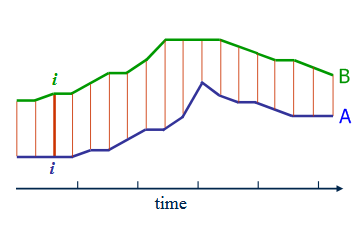
\includegraphics[width=.9\linewidth]{euclidean.png}
		\caption{Distanza Euclidea (lineare)}
		\label{fig:distance_euclidean}
	\end{subfigure}%
	\begin{subfigure}{.5\textwidth}
		\centering
		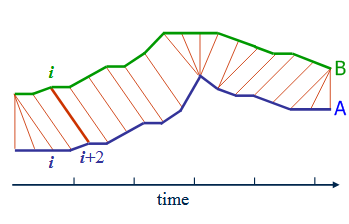
\includegraphics[width=.9\linewidth]{dtw.png}
		\caption{DTW (elastica)}
		\label{fig:distance_dtw}
	\end{subfigure}
	\caption{Confronto tra distanza Euclidea e DTW}
	\label{fig:distance}
\end{figure}
In altre parole, il DTW cerca di "allineare" al meglio le due TS, facendo in modo che entrambe proseguano con lo stesso andamento.\\
\\
La similarità del DTW produce buoni risultati per le TS che rappresentano uno stesso evento ma che sono di lunghezza differente, ad esempio quando entra in gioco uno sfasamento temporale.\\
Un individuo che pronuncia una stessa frase con lo stesso tono ma con velocità differente produrrebbe due TS molto differenti che se si confrontassero linearmente non si riuscerebbe a riconoscere lo stesso individuo, che altrimenti sarebbe possibile se si confrontassero con il DTW.\\
\\
L'algoritmo compie una ricerca nella matrice di distanza, di spazio $O(mn)$, dove $m$ ed $n$ sono le lunghezze delle due TS confrontate.\\
Richiede, quindi, molto tempo al caso pessimo e in letteratura sono state definite alcune implementazioni veloci, come \textit{PrunedDTW}, \textit{SparseDTW} e \textit{FastDTW}, ma nonostante ciò, la tecnica resta complessa in tempo e spazio in caso di dataset ad alta dimensionalità.\\

\section{Confronto con k-Means di TSLearn}
Tramite la libreria TSLearn è stato possibile effettuare il clustering \textbf{k-Means usando come metrica di distanza DTW} sulle TS originale, cioè non ridotte di dimensionalità.\\
Chiaramente, essendo FordA, FordB e RefrigerationDevices dataset ad alta dimensionalità, è stato possibile effettuare il clustering solo per un sottoinsieme dei sample poiché il tempo richesto da DTW per calcolare le matrici di distanza è troppo.\\
\\
+++ ALTRI DETTAGLI MANUEL++++\\
\\
Di seguito sono riportati i risultati del clustering dei dataset in esame, con però alcune premesse:
\begin{itemize}
	\item Non è riportata il Silhouette Coefficient perché essa richiede il calcolo della distanza DTW per ogni coppia di test sample, quindi il tempo richiesto è ancora più alto del tempo richiesto dal k-Means;
	\item Non viene riportata la Relative Purity perché introdotta in un secondo momento, quando i risultati di TSLearn erano stati già calcolati e ricalcolarli avrebbe richiesto molto tempo;
	\item Il k per k-Means è pari al numero di classi presenti nel dataset;
\end{itemize}

\subsubsection{ECG5000}
\begin{center}
	\pgfplotstabletypeset[
	col sep=comma,
	string type,
	every head row/.style={
		before row={\hline
			\multicolumn{2}{c|}{\textbf{ECG5000}} &
			\multicolumn{1}{c|}{Internal} & \multicolumn{3}{c}{External} \\
		},
		after row=\hline
	},
	every last row/.style={after row=\hline},
	]{metrics/dtw/ECG5000_dtw.csv}
	\begin{table}[H]
		\centering
		\caption{5-Means con DTW su ECG5000. \textbf{Gli score dell'autoencoder sono molto simili a questi}. L'autoencoder è allora riuscito ad estrarre bene le caratteristiche degli elettrocardiogrammi, come intuito dall'analisi precedente.}
	\end{table}
\end{center}

\subsubsection{ECG200}
\begin{center}
	\pgfplotstabletypeset[
	col sep=comma,
	string type,
	every head row/.style={
		before row={\hline
			\multicolumn{2}{c|}{\textbf{ECG200}} &
			\multicolumn{1}{c|}{Internal} & \multicolumn{3}{c}{External} \\
		},
		after row=\hline
	},
	every last row/.style={after row=\hline},
	]{metrics/dtw/ECG200_dtw.csv}
	\begin{table}[H]
		\centering
		\caption{2-Means con DTW su ECG200. \textbf{Gli score dell'autoencoder con 2-Means sono migliori rispetto a questi}. La causa potrebbe essere la dimensione ridotta del dataset che non ha permesso TSLearn di operare bene.}
	\end{table}
\end{center}

\subsubsection{ChlorineConcentration}
\begin{center}
	\pgfplotstabletypeset[
	col sep=comma,
	string type,
	every head row/.style={
		before row={\hline
			\multicolumn{2}{c|}{\textbf{Chlorine}} &
			\multicolumn{1}{c|}{Internal} & \multicolumn{3}{c}{External} \\
		},
		after row=\hline
	},
	every last row/.style={after row=\hline},
	]{metrics/dtw/ChlorineConcentration_dtw.csv}
	\begin{table}[H]
		\centering
		\caption{3-Means con DTW su ChlorineConcentration. \textbf{Gli score dell'autoencoder con 3-Means sono quasi identici a questi}. L'autoencoder è allora riuscito ad estrarre bene le caratteristiche di queste TS, cosa non colta durante l'analisi precedente.}
	\end{table}
\end{center}

\subsubsection{FordA}
\begin{center}
	\pgfplotstabletypeset[
	col sep=comma,
	string type,
	every head row/.style={
		before row={\hline
			\multicolumn{2}{c|}{\textbf{FordA}} &
			\multicolumn{1}{c|}{Internal} & \multicolumn{3}{c}{External} \\
		},
		after row=\hline
	},
	every last row/.style={after row=\hline},
	]{metrics/dtw/FordA_dtw.csv}
	\begin{table}[H]
		\centering
		\caption{2-Means con DTW su FordA. ++++TODO++++}
	\end{table}
\end{center}

\subsubsection{FordB}
\begin{center}
	\pgfplotstabletypeset[
	col sep=comma,
	string type,
	every head row/.style={
		before row={\hline
			\multicolumn{2}{c|}{\textbf{FordB}} &
			\multicolumn{1}{c|}{Internal} & \multicolumn{3}{c}{External} \\
		},
		after row=\hline
	},
	every last row/.style={after row=\hline},
	]{metrics/dtw/FordB_dtw.csv}
	\begin{table}[H]
		\centering
		\caption{2-Means con DTW su FordB. ++++TODO++++}
	\end{table}
\end{center}

\subsubsection{PhalangesOutlineCorrect}

\subsubsection{RefrigerationDevices}
\begin{center}
	\pgfplotstabletypeset[
	col sep=comma,
	string type,
	every head row/.style={
		before row={\hline
			\multicolumn{2}{c|}{\textbf{RefrigerationDevices}} &
			\multicolumn{1}{c|}{Internal} & \multicolumn{3}{c}{External} \\
		},
		after row=\hline
	},
	every last row/.style={after row=\hline},
	]{metrics/dtw/RefrigerationDevices_dtw.csv}
	\begin{table}[H]
		\centering
		\caption{3-Means con DTW su RefrigerationDevices. ++++TODO++++}
	\end{table}
\end{center}

\subsubsection{TwoLeadECG}

\subsubsection{TwoPatterns}

\section{Confronto con altre tecniche di feature extraction and selection}
Sono stati reperiti alcuni risultati di clustering sui dataset in esame attuando però altre tecniche di feature extraction and selection. Il clustering è stato fatto con k-Means con k pari al numero di classi del dataset e su un numero differente di feature estratte in modo diverso:
\begin{itemize}
	\item Tutte le feature estratte da \textbf{TSFresh};
	\item Feature rilevanti selezionate da TSFresh;
	\item Feature rilevanti selezionate dall'algoritmo \textbf{NDFS};
	\item Feature rilevanti selezionate dall'algoritmo \textbf{Lap Score}.
\end{itemize}
Degli score riportati nelle seguenti tabelle, solamente silhouette, Davies-Bouldin e purity verranno usate per il confronto.

\subsubsection{ECG5000}
\begin{figure}[H]
	\centering
	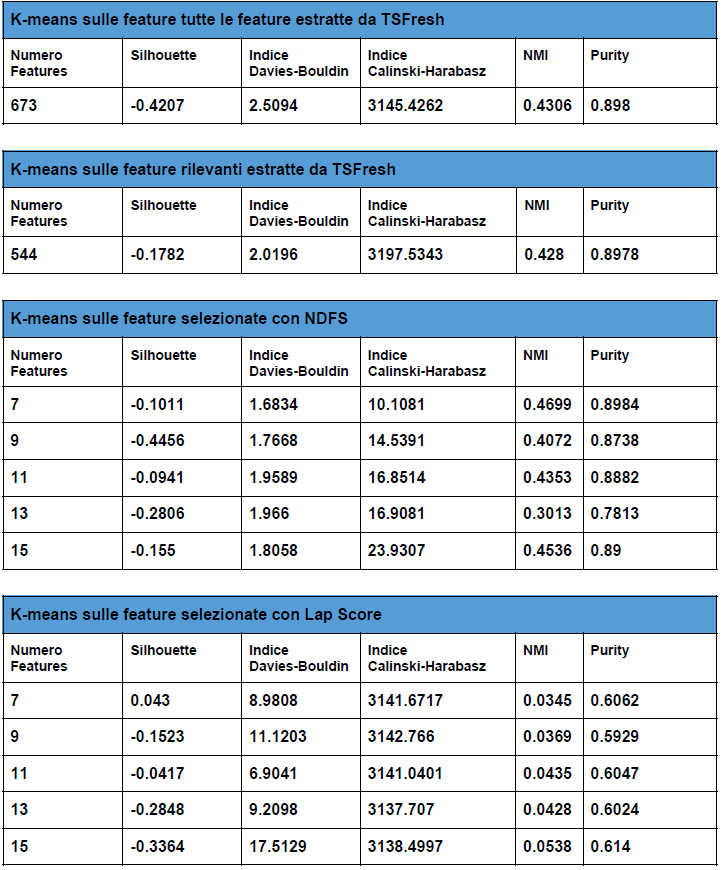
\includegraphics[width=\linewidth]{av/ecg5000_av.png}
	\caption{ECG5000 con tecniche di feature extraction and selection. TSFresh ed NDFS riportano DB e purity simili a quelli dell'autoencoder, mentre LapScore inizia a peggiorarli di molto. L'autoencoder ha migliore silhouette in ogni caso.}
	\label{fig:ecg5000_av}
\end{figure}

\subsubsection{ECG200}
\begin{figure}[H]
	\centering
	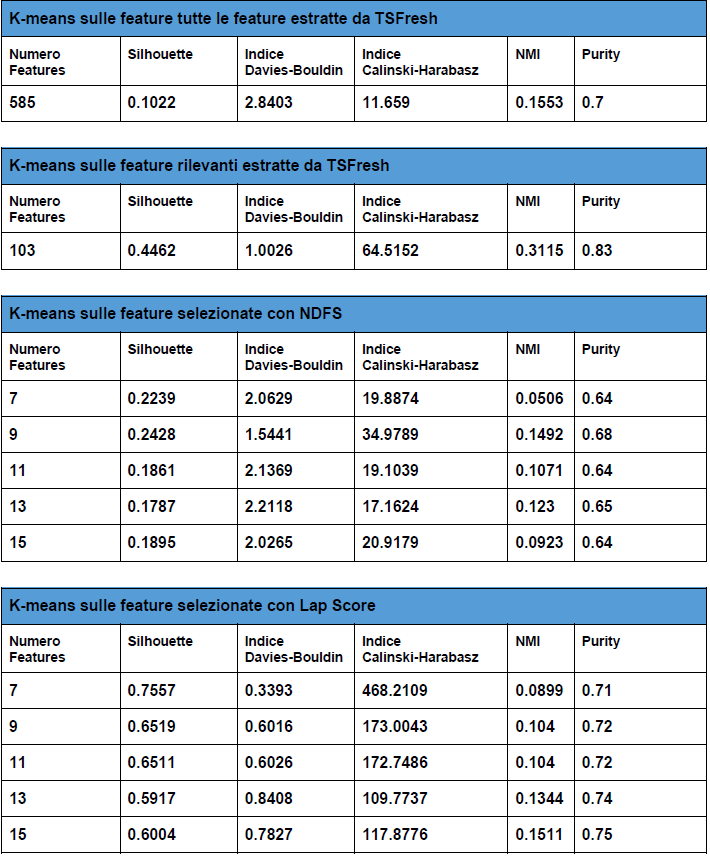
\includegraphics[width=\linewidth]{av/ecg200_av.png}
	\caption{ECG200 con tecniche di feature extraction and selection. La purity è molto simile ai risultati dell'autoencoder. La silhouette dell'autoencoder è migliore rispetto a TSFresh e NDFS, ma peggiore rispetto a Lap Score. Analogo discorso per DB, eccetto che per le feature rilevanti di TSFresh è molto simile.}
	\label{fig:ecg200_av}
\end{figure}

\subsubsection{ChlorineConcentration}
\begin{figure}[H]
	\centering
	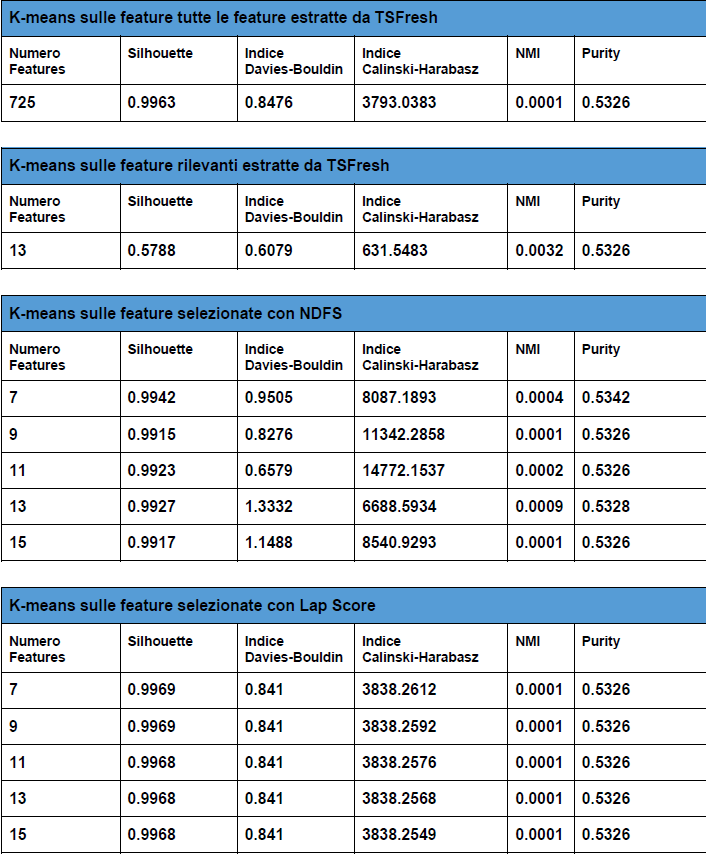
\includegraphics[width=\linewidth]{av/chlorine_av.png}
	\caption{ChlorineConcentration con tecniche di feature extraction and selection. La silhouette ritornata dall'autoencoder è peggiore, in particolar modo rispetto ad NDFS e Lap Score, mentre il DB è simile, alternando casi in cui l'autoencoder vince rispetto a qualche tecnica. La purity è pressocché indentica per tutti.}
	\label{fig:chlorine_av}
\end{figure}

\subsubsection{FordA}
\begin{figure}[H]
	\centering
	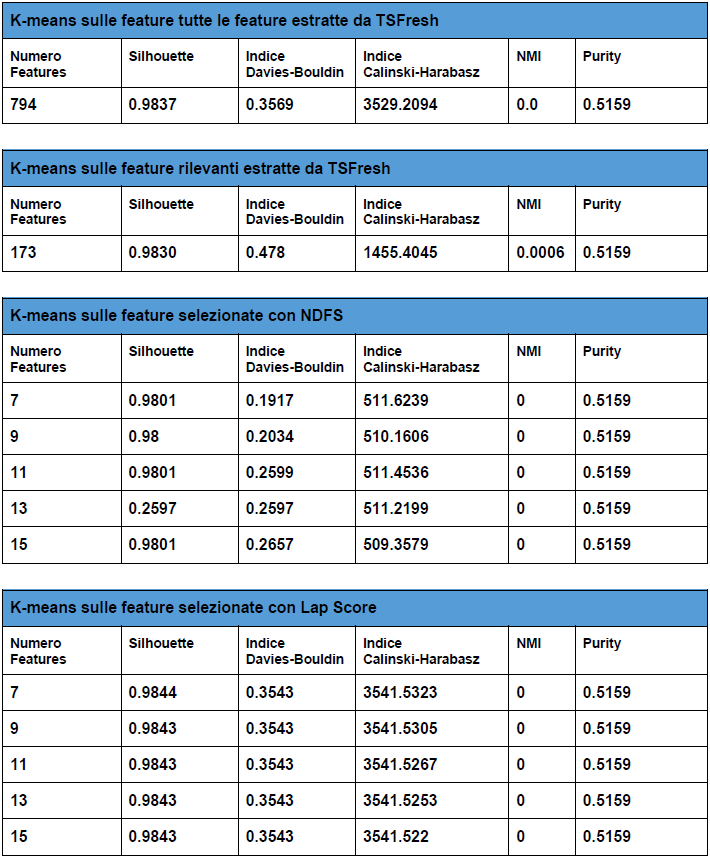
\includegraphics[width=\linewidth]{av/forda_av.png}
	\caption{FordA con tecniche di feature extraction and selection. +++TODO+++}
	\label{fig:forda_av}
\end{figure}

\subsubsection{FordB}
\begin{figure}[H]
	\centering
	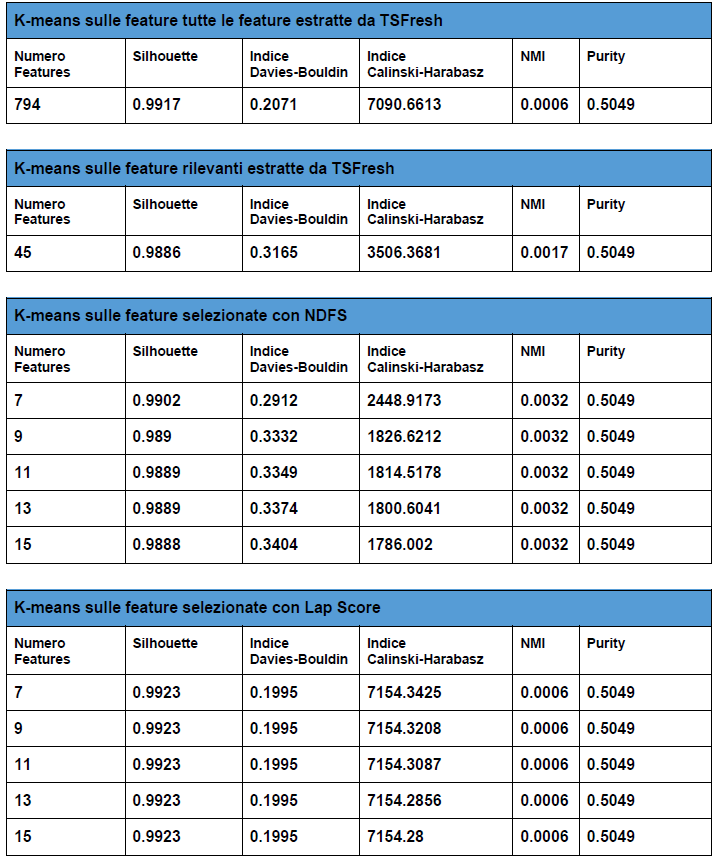
\includegraphics[width=\linewidth]{av/fordb_av.png}
	\caption{FordB con tecniche di feature extraction and selection. +++TODO+++}
	\label{fig:fordb_av}
\end{figure}

\subsubsection{PhalangesOutlineCorrect}
\begin{figure}[H]
	\centering
	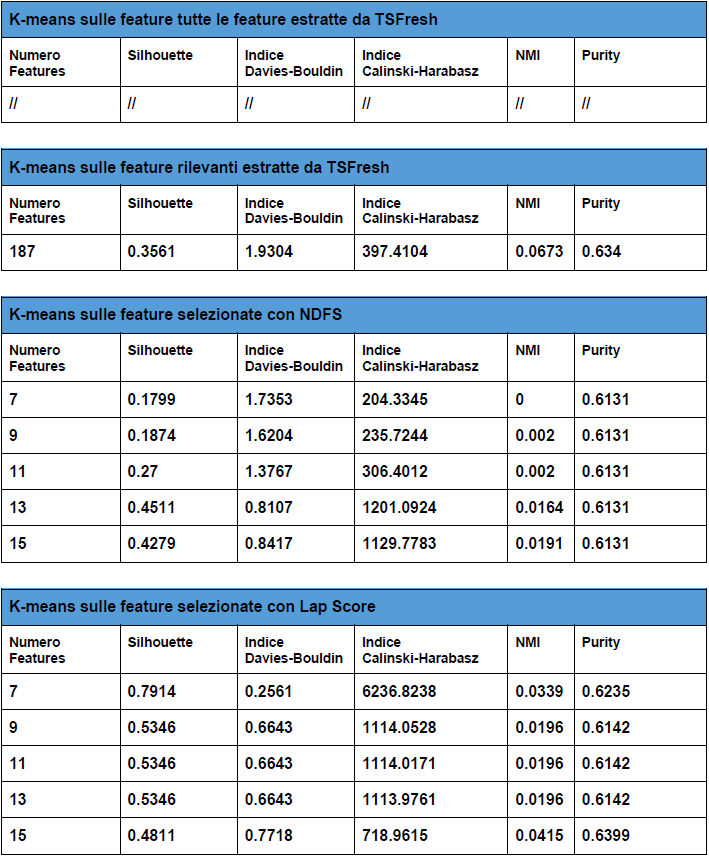
\includegraphics[width=\linewidth]{av/phalanges_av.png}
	\caption{PhalangesOutlineCorrect con tecniche di feature extraction and selection. Silhouette e DB sono variabili: qualche volta sono migliori nell'autoencoder (caso TSFresh e una parte di NDFS), altre volte è peggiore (caso Lap Score e l'altra parte di NDFS). La purity è pressocché identica in tutti i casi.}
	\label{fig:phalanges_av}
\end{figure}

\subsubsection{RefrigerationDevices}
\begin{figure}[H]
	\centering
	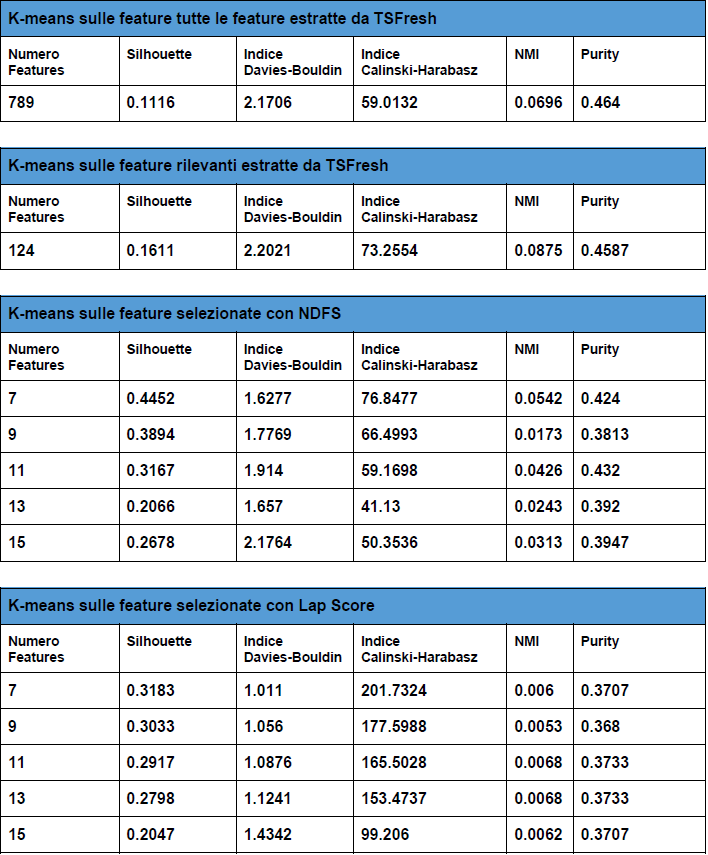
\includegraphics[width=\linewidth]{av/refrigeration_av.png}
	\caption{RefrigerationDevices con tecniche di feature extraction and selection. +++TODO+++}
	\label{fig:refrigeration_av}
\end{figure}

\subsubsection{TwoLeadECG}
\begin{figure}[H]
	\centering
	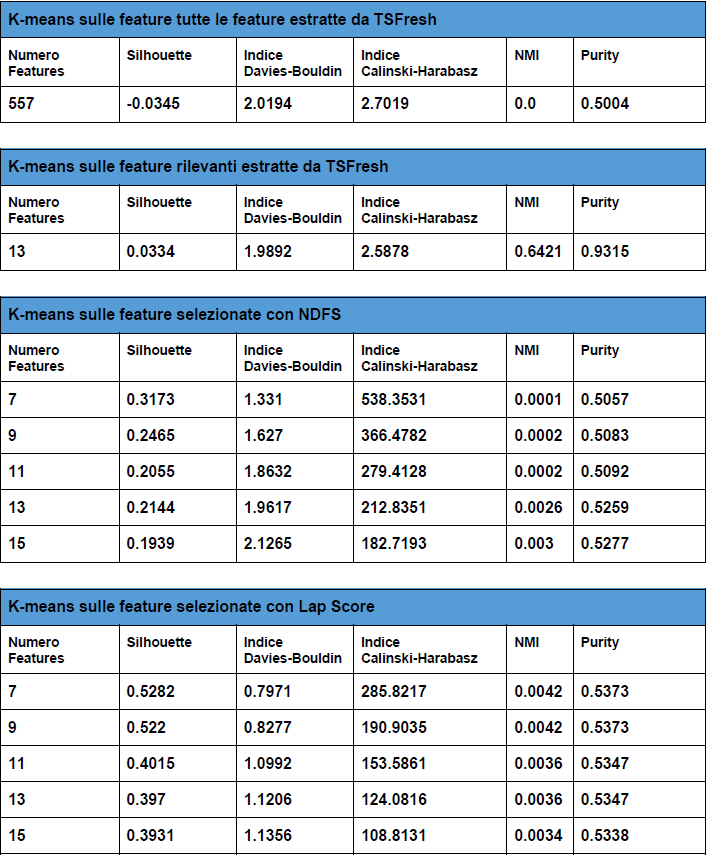
\includegraphics[width=\linewidth]{av/twoleadecg_av.png}
	\caption{TwoLeadECG con tecniche di feature extraction and selection. Silhouette e DB dell'autoencoder sono leggermente peggiori delle migliori silhouette e DB ottenuti in una delle esecuzioni di Lap Score, quindi mediamente l'autoencoder ha avuto score migliori. La purity è pressocché identica in tutti i casi eccetto il caso delle feature rilevanti di TSFresh dove è nettamente superiore.}
	\label{fig:twoleadecg_av}
\end{figure}

\subsubsection{TwoPatterns}
\begin{figure}[H]
	\centering
	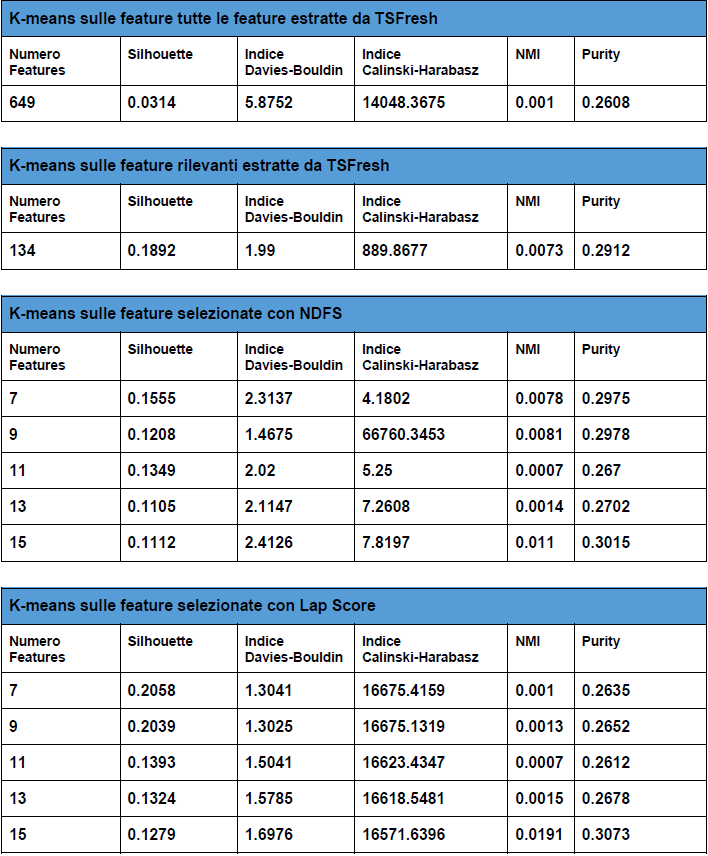
\includegraphics[width=\linewidth]{av/twopatterns_av.png}
	\caption{TwoPatterns con tecniche di feature extraction and selection. Sebbene quella dell'autoencoder sia una delle silhouette peggiori, è in generale molto bassa in tutti i casi, quindi potrebbe essere molto legato alla natura dei dati o di k-Means. Analogo ragionamento per DB. La purity è molto simile in tutti i casi, sebbene non siano ottimi valori.}
	\label{fig:twopatterns_av}
\end{figure}